\documentclass{beamer}



\usepackage{listings}
\usepackage[english]{babel}
\usepackage{amsmath}
\usepackage[latin1]{inputenc}
\usepackage{units}
\usepackage{colortbl}
\usepackage{multimedia}
\usepackage{bm}
\usepackage{subcaption}
\usepackage{algorithm2e}
\usepackage{algorithmic}

% Math commands
\newcommand{\sys}{S}
\newcommand{\diss}{d}
\newcommand{\learn}{\mathcal{A}}
\newcommand{\free}{\mathcal{M}}
\newcommand{\D}{\mathcal{D}}
\newcommand{\R}{\mathbb{R}}
\newcommand{\nsamp}{N}
\newcommand{\norm}[1]{\left\lVert#1\right\rVert}

\newcommand{\E}{\mathbb{E}}
\newcommand{\mdl}{M}
\newcommand{\mdlstruc}{\mathcal{M}}

% Colors
\definecolor{darkgreen}{RGB}{20,150,50}
\definecolor{Periwinkle}{rgb}{0.0, 0.0, 0.0}
\definecolor{darkgreen}{RGB}{20,150,50}
\definecolor{orange}{RGB}{204, 85, 0}

\mode<presentation>
{
  \usetheme{Boadilla}
  \useoutertheme{infolines}
  \setbeamercovered{transparent}
}


\title[In-context learning sysid]{\textsc{On the adaptation of in-context learners for system identification}}


%\author[]{Marco Forgione\inst{1}, Filippo Pura\inst{1}, Dario Piga\inst{1}}
\author[]{Marco Forgione, Filippo Pura, Dario Piga}

\institute[IDSIA]{
	\inst{}IDSIA Dalle Molle Institute for Artificial Intelligence SUPSI-USI, Lugano, Switzerland
	}


\date[SYSID 2024]{SYSID 2024 \\ 17-18 July 2024, Boston, USA}
%\date[]{\today}


\subject{System Identification, Meta Learning, In-context Learning, Transformers}

\newcommand{\book}{
\includegraphics[width=10pt]{fig/proceeding-logo.jpg}}
\newcommand{\github}{
\includegraphics[width=10pt]{fig/github-logo.jpg}}


\begin{document}

\begin{frame}
  \titlepage
\end{frame}



\begin{frame}{Standard system identification/supervised machine learning}
%Standard system identification workflow:
\begin{enumerate}
\item Collect dataset $\D = (u_{1:N}, y_{1:N})$ of input/outputs
%$$\D = u_{1:N}, y_{1:N}$$
from  system $\sys$.
\item Apply an algorithm to estimate a model $M(\hat \theta)$ of $\sys$:
$$\hat \theta = \learn(\D)  \qquad \text{e.g.  }  \learn(\D)  = \mathrm{PEM}$$
%\arg \min_{\theta \in \Theta} \mathcal{L}(\D, M(\theta))$$
\item Make predictions/simulations using the model on new data:
%$$\hat y_k = M(u_{1:k-1}; \theta^*)$$
$$\hat y^*_{1:M} = M(u^*_{1:M}; \hat \theta)$$
\end{enumerate}
\pause
Researchers keep on improving learning algorithms and model structures.\\
Can we automate this process?
Can we \structure{learn the learning algorithm} itself?\\
\pause

\vskip .5em
\structure{Meta learning} tries to answer this question.


 	\begin{itemize}
	\item[\book]
		\begin{tiny}
	\structure{J. Schmidhuber.}
     Evolutionary principles in self-referential learning, or on learning how to learn. \vskip -1em
     \emph{Diploma Thesis, TU Munich, 1987}
		\end{tiny}\\

	\item[\book]
		\begin{tiny}
	\structure{T. Hospedales et al.} % A. Antoniou, P. Micaelli, and A. Strokey
     Meta-Learning in Neural Networks: A Survey.
     \emph{IEEE Transactions on Pattern Analysis and Machine \vskip -1em
      Intelligence, 2022}
		\end{tiny}\\

    \end{itemize}

\end{frame}


\begin{frame}{Our meta learning setting}
\begin{itemize}
%Meta learning setting
 \item We have an \structure{infinite stream} of datasets from a distribution $p(\D)$:
  $$\{\D^{(i)} = (u_{1:\nsamp}^{(i)}, y_{1:\nsamp}^{(i)}), \,\, i=1,2,\dots, \infty \}$$
 \item $\D^{(i)}$ generated by \structure{random system} $\sys^{(i)}$ and input realization $u_{1:\nsamp}^{(i)}$
 \item Different but \structure{related to each other}. There's a learnable structure!
\end{itemize}
\vskip 1em
\pause
Can we get better at identifying $\sys^{(i)}$ as we observe more datasets $\D^{(j)}$?
\pause
\vskip 1em
\begin{itemize}
\item $p(\D)$ may be a \structure{physical simulator} where we can change settings
\item The learned algorithm could then be applied to \structure{real data}
% with insight
\end{itemize}
%\vskip 1em
%\pause
%Meta learning from a \structure{finite collection} would also be interesting...
\end{frame}

\begin{frame}{In-context learning}
Many meta learning strategies around. Here focus on \structure{in-context learning}.
\vskip 1em
%\begin{itemize}
%\item \structure{Transformers} are expressive  as \structure{a programming language}%are sufficiently expressive to \structure{represent algorithms}.
We provide a very powerful ML model (Transformer) with:
\begin{itemize}
\item A \structure{context}, namely an input/output sequence of a system
\item A \structure{task}, like predicting the next output or simulating for more steps
\end{itemize}
The Transformer must \structure{learn to identify} the system to solve the task!
%\end{itemize}
\vskip 1em

\pause

Context + task may be seen as a \structure{prompt} to a Large Language Model, which can then
\structure{continue the word sequence} in an optimal way.
\begin{align*}
	 \text{question} \rightarrow \text{answer}\\
     u_{1:m}, y_{1:m}, u_{m+1:N} \rightarrow \hat y_{m+1:N}
\end{align*}

\begin{itemize}
%	\item[\book]
%		\begin{tiny}
%	\structure{G.~Weiss et al.} 
%     Thinking like Transformers.
%     \emph{38th International Conference on Machine Learning (ICML 2022).}
%		\end{tiny}
		
	\item[\book]
		\begin{tiny}
	\structure{S. Garg et al.} % A. Antoniou, P. Micaelli, and A. Strokey
     What Can Transformers Learn In-Context? A Case Study of Simple Function Classes.
     \emph{36th Conference on \vskip -1em Neural Information Processing Systems (NeurIPS 2022).}
		\end{tiny}

	\item[\book]
		\begin{tiny}
	\structure{T. Brown et al.} % A. Antoniou, P. Micaelli, and A. Strokey
     Language Models are Few-Shot Learners.
     \emph{34th Conference on  Neural Information Processing Systems \vskip -1em (NeurIPS 2020).}
		\end{tiny}\\

\end{itemize}
\end{frame}


\begin{frame}{In-context learning with Transformers}
%     \begin{columns}[t]
%     \column{.48\textwidth}
%     \begin{block}{Multi-step simulation}
%     \vskip -1em
%     Meta-model trained to predict $\hat y_{m+1:N} = \free_\phi(u_{1:m}, y_{1:m}, u_{m+1:N})$
     %\vskip .8em
     %Meta-model receives:
     \begin{itemize}
     \item Full I/O sequence $(u_{1:m}, y_{1:m})$ characterizes the dynamics (context)
     \item Input squence $u_{m+1:N}$ defines the simulation objective (task) 
     \end{itemize}
     \begin{figure}
          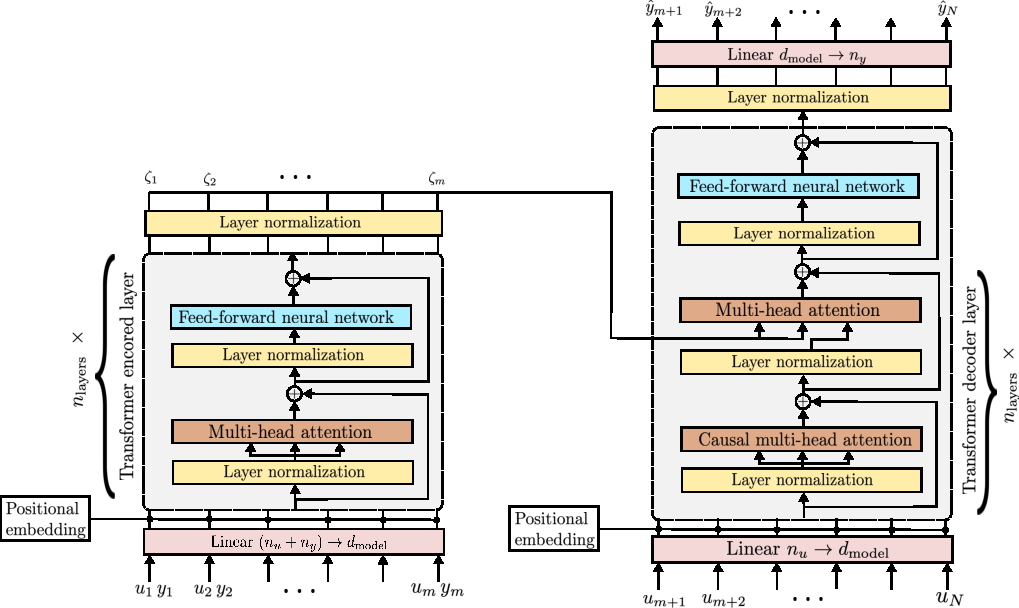
\includegraphics[height=150 pt]{fig/architecture/encoder_decoder_architecture.pdf}
          %encoder-decoder ($\sim$ language translation)
     \end{figure}
     %\vskip 1em
     %and generates simulation:
     %$\hat y_{m+1:N}$
     %\vskip 1em
     %\begin{itemize}
     %\item $u_{1:m}, y_{1:m}, u_{m+1:N} \rightarrow \hat y_{m+1:N}$
     %\end{itemize}
%     \end{block}
%     \end{columns}
     \pause
     %\vskip 1em
     \begin{itemize}
     \item The Transformer $\free_\phi$  becomes a  \structure{meta model} of the system class!
     \item $ \free_\phi$ becomes \structure{as powerful as a system identification algorithm}!
     \end{itemize}
     \end{frame}
     
\begin{frame}{Meta model training}
Meta model $\free_\phi$ trained in a standard \structure{supervised learning} setting: 
\begin{small}
     $$\hat \phi = \arg \min_\phi \mathcal{L}_{\rm sim}(\phi)$$
\begin{align*}
     \mathcal{L}_{\rm sim}(\phi)   &=   \E_{p(\D)}
     \left [
     \norm{y_{m+1:\nsamp} \! - \! \free_\phi (u_{1:m}, y_{1:m}, u_{m+1:\nsamp})
     }^2
     \right ] \\
      & \approx
     \frac{1}{b}
     \sum_{i=1}^b
     %
     \norm{y_{m+1:\nsamp}^{(i)} - \free_\phi (u_{1:m}^{(i)}, y_{1:m}^{(i)}, u_{m+1:\nsamp}^{(i)})}^2
\end{align*}
\end{small}

\pause
\begin{itemize}
\item Training \structure{on a whole class} of dynamical systems
makes the outcome special.
\item If the optimization works out well, the Transformer becomes a \structure{meta model} of the systems in $p(\D)$.
\item We have \structure{learned a learning algorithm!}
\end{itemize}
\end{frame}


\begin{frame}{Previous experiments - System classes}
One-step prediction and multi-step simulation on two system classes:
%\vskip 1em
\begin{columns}[t]

\column{.48\textwidth}
\begin{block}{Linear Time Invariant (LTI):}
In state-space form, order $\leq 10$
\begin{align*}
x_{k+1} &= Ax_k + Bu_k\\
y_{k+1} &= Cx_k
\end{align*}
\vskip -.5em
\begin{itemize}
\item Random system matrices
\item $A$ constrained to be stable
\end{itemize}
\end{block}
\column{.48\textwidth}
\begin{block}{Wiener-Hammerstein (WH):}
\vskip .8em
\begin{figure}
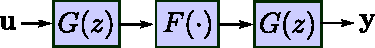
\includegraphics[width=.7\textwidth]{fig/wiener_hammerstein.pdf}
\end{figure}
\begin{itemize}
\item Sequential LTI $\rightarrow$ $F(\cdot)$ $\rightarrow$ LTI
\item Random LTI, order $\leq 5$
\item $F(\cdot)$: random feedforward NN.
\end{itemize}
\end{block}
\end{columns}
\vskip 1em
\begin{itemize}
\item For both classes, input $u_{1:\nsamp}$ is a white Gaussian noise sequence.
\item This defines a $p(\D)$. We can generate infinite datasets!
\item Each dataset from a different input/system realization!
\end{itemize}

 	\begin{itemize}
	\item[\github]
		\begin{tiny}
          M. Forgione, F. Pura, D. Piga. In-context learning for model-free system identification. IEEE Control Systems Letters, \vskip -1em 2023
		%\url{https://github.com/forgi86/sysid-transformers}
		\end{tiny}\\
 \end{itemize}
\end{frame}

\begin{frame}{Previous experiments - multi-step simulation results}
\begin{columns}[t]
\column{.5\textwidth}
\begin{center}
\begin{figure}
LTI: one sequence
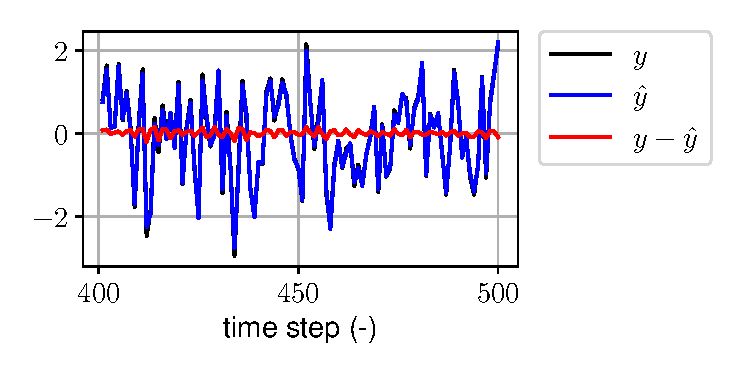
\includegraphics[width=\textwidth]{fig/lin_sim_single.pdf}
WH: one sequence
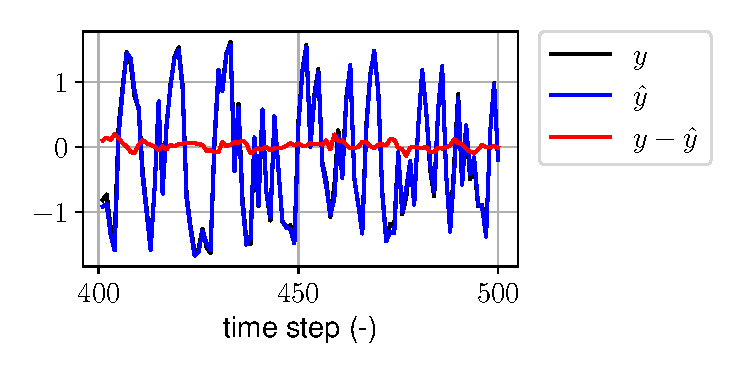
\includegraphics[width=\textwidth]{fig/wh_sim_single.pdf}
\end{figure}
\end{center}
\column{.5\textwidth}
\begin{center}
\begin{figure}
LTI: 256 sequences
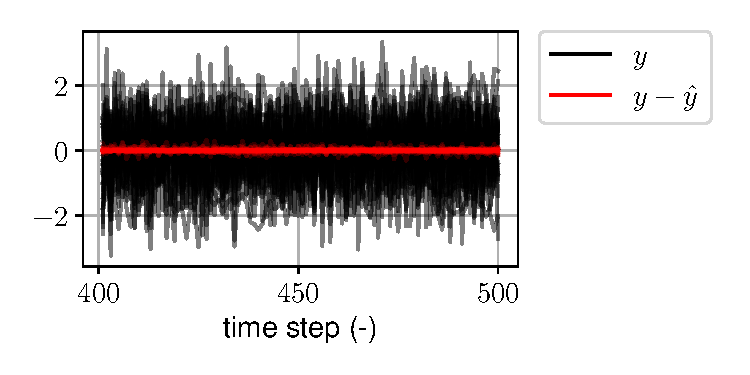
\includegraphics[width=\textwidth]{fig/lin_sim_batch.pdf}
WH: 256 sequences
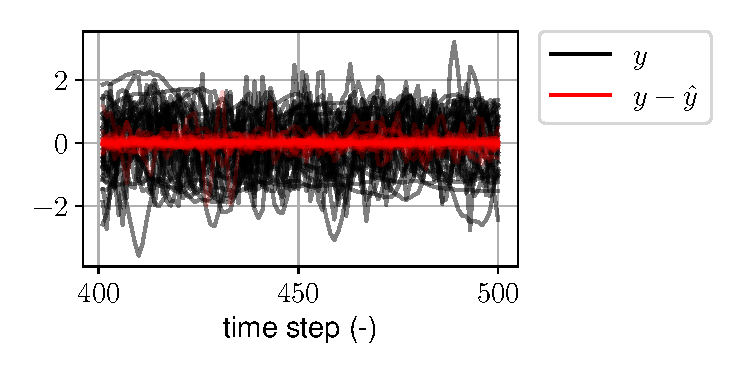
\includegraphics[width=\textwidth]{fig/wh_sim_batch.pdf}
\end{figure}
\end{center}
\end{columns}
\end{frame}

\begin{frame}{New experiments - Generalization and adaptation}
Training meta models from scratch is relatively expensive and data hungry.
\begin{itemize}
 \item For the WH class, $\approx$ 1 day on a 3090 GPU over 32M training instances.
\end{itemize}
\pause
\vskip 1em
     In this SYSID '24 work, we investigate:
     \begin{enumerate}
          \item \structure{Generalization} of a trained meta model on a \structure{new system class}
          \item \structure{Adaptation} of a meta model to:
          \begin{enumerate}
               \item A {specific instance} within the system class (specialization)
               \item A {system instance} outside of the system class
               %\item New system classes. From WH to Parallel WH with multiple branches
               \item New tasks. From 100- to 1000-step-ahead simulation
          \end{enumerate}

     \end{enumerate}
\end{frame}

\begin{frame}{Generalization}
Three LTI system classes. Order $< 10$, eigs with mag/phase in ranges:
\begin{columns}
\column{.5\textwidth}
\begin{itemize}
     \item[a] $(0.8, 0.97) / (-\nicefrac{\pi}{2}, \nicefrac{\pi}{2})$
     \item[b] $(0.5, 0.75) / (\nicefrac{\pi}{2}, \nicefrac{3}{4}\pi)$
     \item[c] $(0.5, 0.97) / (-\pi, \pi)$  
\end{itemize}
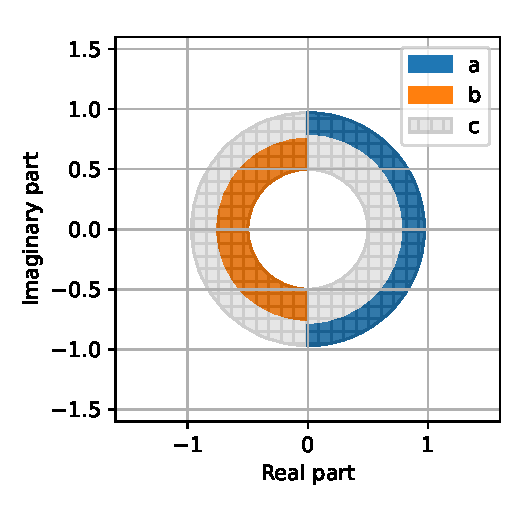
\includegraphics[height=100pt]{fig/shift/pole_distribution.pdf}
\column{.5\textwidth}
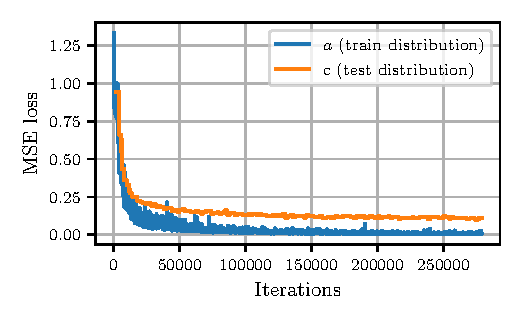
\includegraphics[height=75pt]{fig/shift/loss_shift_A.pdf}\\
%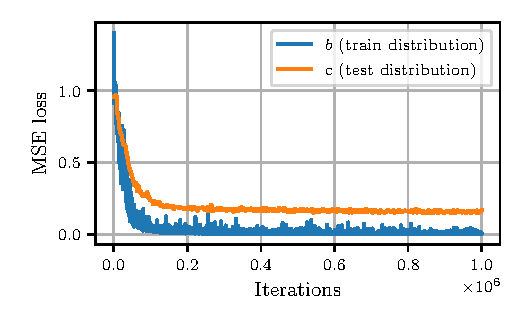
\includegraphics[height=50pt]{fig/shift/loss_shift_B.pdf}\\
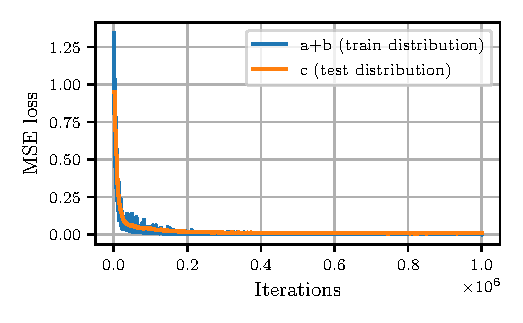
\includegraphics[height=75pt]{fig/shift/loss_shift_AB.pdf}
\end{columns}
\pause
\begin{itemize}
     \item Training only on a or b leads to a large generalization error on c.
     \item Training on a+b leads to a small generalization error on c
     \item Good generalization to unseen regions (gray area)
\end{itemize}

\end{frame}

\begin{frame}{Adaptation to specific system instances}
With just 140 sequences and $\approx$ 5 minutes of fine-tuning we can adapt, the WH meta model:
\begin{itemize}
     \item To a specific instance of the WH class (left)
     \item To a PWH system instance, which is out of the WH class (right)
\end{itemize}

\begin{columns}
\column{.5\textwidth}
\begin{figure}
     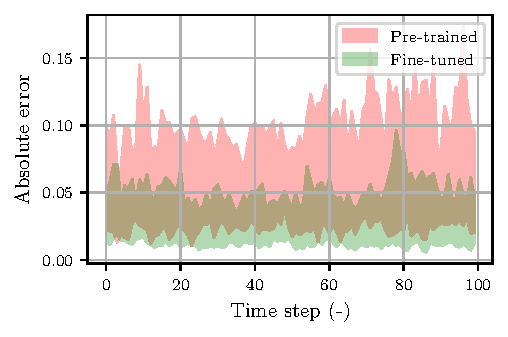
\includegraphics[height=100pt]{fig/adaptation/wh_error_25_75_percentile.pdf}
\end{figure}
\column{.5\textwidth}
\begin{figure}
     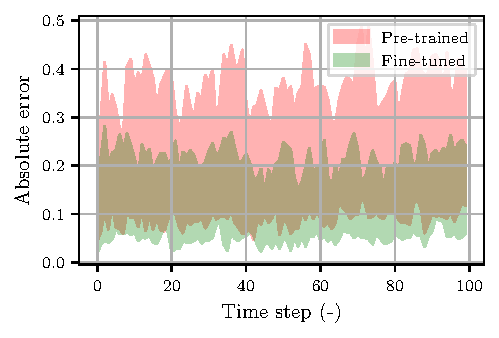
\includegraphics[height=100pt]{fig/adaptation/pwh_error_25_75_percentile.pdf}
\end{figure}
\end{columns}
\pause
\vskip 1em
REMARK: training the WH meta model from scratch required instead $\approx$  32M training instances and took
1 day!
\end{frame}

\begin{frame}{Adaptation to new tasks}
     We try to learn a 1000-step-ahead meta model for the WH class.
     \begin{figure}
     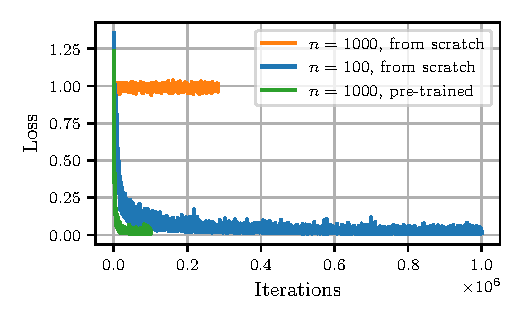
\includegraphics[height=100pt]{fig/short_long/wh_pretrain_iterations.pdf}
     \end{figure}
     \begin{itemize}
          \item Learning the 1000-step model from scratch (orange) seems hard. Loss is stuck at a high value
          \item Learning a 100-step model (blue) is possible. We also did it in our previous work...
          \item Starting from the 100-step model, the optimization of the 1000-step model converges very quickly (green line)!
     \end{itemize}
\end{frame}

\begin{frame}{Conclusions}
\begin{itemize}
\item While training of a meta-model from scratch is computationally intensive, adaptation to new tasks and systems is fast and efficient.
\item This makes the case for the development of \structure{foundation models} for system identification.
\end{itemize}
%  Further investigations on \structure{in-context} learning approach for system identification.
%  \begin{itemize}
%   \item Model-free, no need to re-train for a specific dataset/system
%   \item Exploits the power of Transformers seen as \structure{trainable algorithms}
%   \item Seems to work!
%  \end{itemize}
%  \pause
%  \vskip 1em
\pause
\vskip 1em
Many possible research directions and applications including:
 \begin{itemize}
  \item State estimation
  \item Control
  \item Dataset augmentation
 \end{itemize}
\end{frame}


\begin{frame}{}{}
\begin{center}
\huge{\structure{Thank you.\\ Questions?}}\\
\vskip 1em
\begin{small}
\texttt{marco.forgione@idsia.ch}
\end{small}
\end{center}
\end{frame}

\end{document}
